\documentclass[conference]{IEEEtran}
\IEEEoverridecommandlockouts
% The preceding line is only needed to identify funding in the first footnote. If that is unneeded, please comment it out.
\usepackage{cite}
\usepackage{amsmath,amssymb,amsfonts}
\usepackage{algorithmic}
\usepackage{graphicx}
\usepackage{textcomp}
\usepackage{xcolor}
\usepackage{url}
\def\BibTeX{{\rm B\kern-.05em{\sc i\kern-.025em b}\kern-.08em
    T\kern-.1667em\lower.7ex\hbox{E}\kern-.125emX}}
\begin{document}

\title{Emotional Recognition on Twitter\\
{\footnotesize CPSC 571 Group 14}
}

\author{\IEEEauthorblockN{1\textsuperscript{st} Matthew Forman}
\IEEEauthorblockA{\textit{dept. Computer Science} \\
\textit{University of Calgary}\\
Calgary, Canada \\
matthew.forman@ucalgary.ca}
\and
\IEEEauthorblockN{2\textsuperscript{nd} Firoz Lakhani}
\IEEEauthorblockA{\textit{dept. Computer Science} \\
\textit{University of Calgary}\\
Calgary, Canada \\
firoz.lakhani1@ucalgary.ca}
\and
\IEEEauthorblockN{3\textsuperscript{rd} Rohan Chaudhary}
\IEEEauthorblockA{\textit{dept. Computer Science} \\
\textit{University of Calgary}\\
Calgary, Canada \\
rohan.chaudhary@ucalgary.ca}
}

\maketitle

\begin{abstract}
This report is going to cover the implemenation of an algoirthm that is used to determine the sentiment and emotion behind a given tweet.
We will discuss the pros and cons of existing methods and how a hybrid of these existing methods could create a more accurate result.
Social media is a space which is utilized to express many sentiments and emotions. 
In many real world applications, it is important to identify these emotions efficiently and as accurately as possible. 
The ability to identify and predict emotional tone and public perception of various issues can be useful in many scenarios. 
For example, being able to differentiate between sarcasm and a person being serious on twitter can be difficult at times. 
With accurate emotional recognition algorithms, one may be able to understand when something is sarcasm vs when it is not and avoid some of the stress and anger a post may instill otherwise. 
As well, there is incentive from large corporations and governments to understand how the public is perceiving a new product or service. 
With this new knowledge products and services could theoretically be changed to help positively effecrt the most amount of people. 

\end{abstract}

\begin{IEEEkeywords}
Insert terms here
\end{IEEEkeywords}

\section{Literature Review}
There are many current studies that have also had intentions to create an algorithm to assign sentiment to tweets.  
From these studies, the following has been discovered.
Assigning sentiment should be split up into three categories, positive, neutral, and negative.
This separation of tweets has been used in several sentiment analysis studies.
For example this was the way tweets were separated in a study by Samah Jailani, Hamzah, Amunuddin, Abidin, and Riza in wich there algorithm "establishes whether a particulartweet is supportive, critical, or neutral\cite{b2}."
Emotion can also be assigned to tweets, these being split up into sections of anger, sadness, joy, fear, and disgust. 
In a study by Benrouba, and Boudour, IBM's natural language understanding API tool was used to analyze words associated with positive, negative and neutral emotions\cite{b1}.
This tools assings values between 0 and 1 for emotions mentioned above per word. 
From here tweets were analyzed to calculate distance to these baseline words in an unsupervised fashion in order to identify the sentiment behind it. 
As well, there was implemenations of this algorithm that focussed on desiphering the sentiment or emotion of a tweet on an individual scale or on a more mass tweet scale.
The analysis in bulk was done mainly to understand how the public was percieving a certain topic of interest online. 
Whereas the individual assessment was more focussed on understanding how one person felt in general based on the sentiment behind their tweets. 
Through analyzing existing papers some pros and cons with exisiting methodologies were established. \newline
\newline
Pros: 
\begin{itemize}
    \item Already established accuracy levels of some existing machine learning algorithms for predicting tweet sentiment.
    \item Proven accuracy of SVM (Support Vector Machine) algoirthm.
\end{itemize}
Cons:
\begin{itemize}
    \item Much fewer studies in which unsupervised algoirthms were tested in this context.
    \item There is a lot of overlap between neurtal, and positive and negative key words making it harder to determine sentiment.
\end{itemize}

As mentioned above, Taking an SVM approach was one of the most accurate in terms of supervised algorithms.
It out performed other algorithms of Sentiment Analysis accross multiple examined studies. 
An SVM works by indentifying "a hyperplane that distinguishably segregates the data points of differnt classes \cite{b6}." 
What this means is the data is expanded onto a multidimensional plane that is split up by the hyperplane. 
The hyperplane will have margins that expand to the size of the closest datapoint to it that falls immediately after the hyplane centre. 
This makes decision making faster and more effiecient. 
\begin{figure}[t]
    \centerline{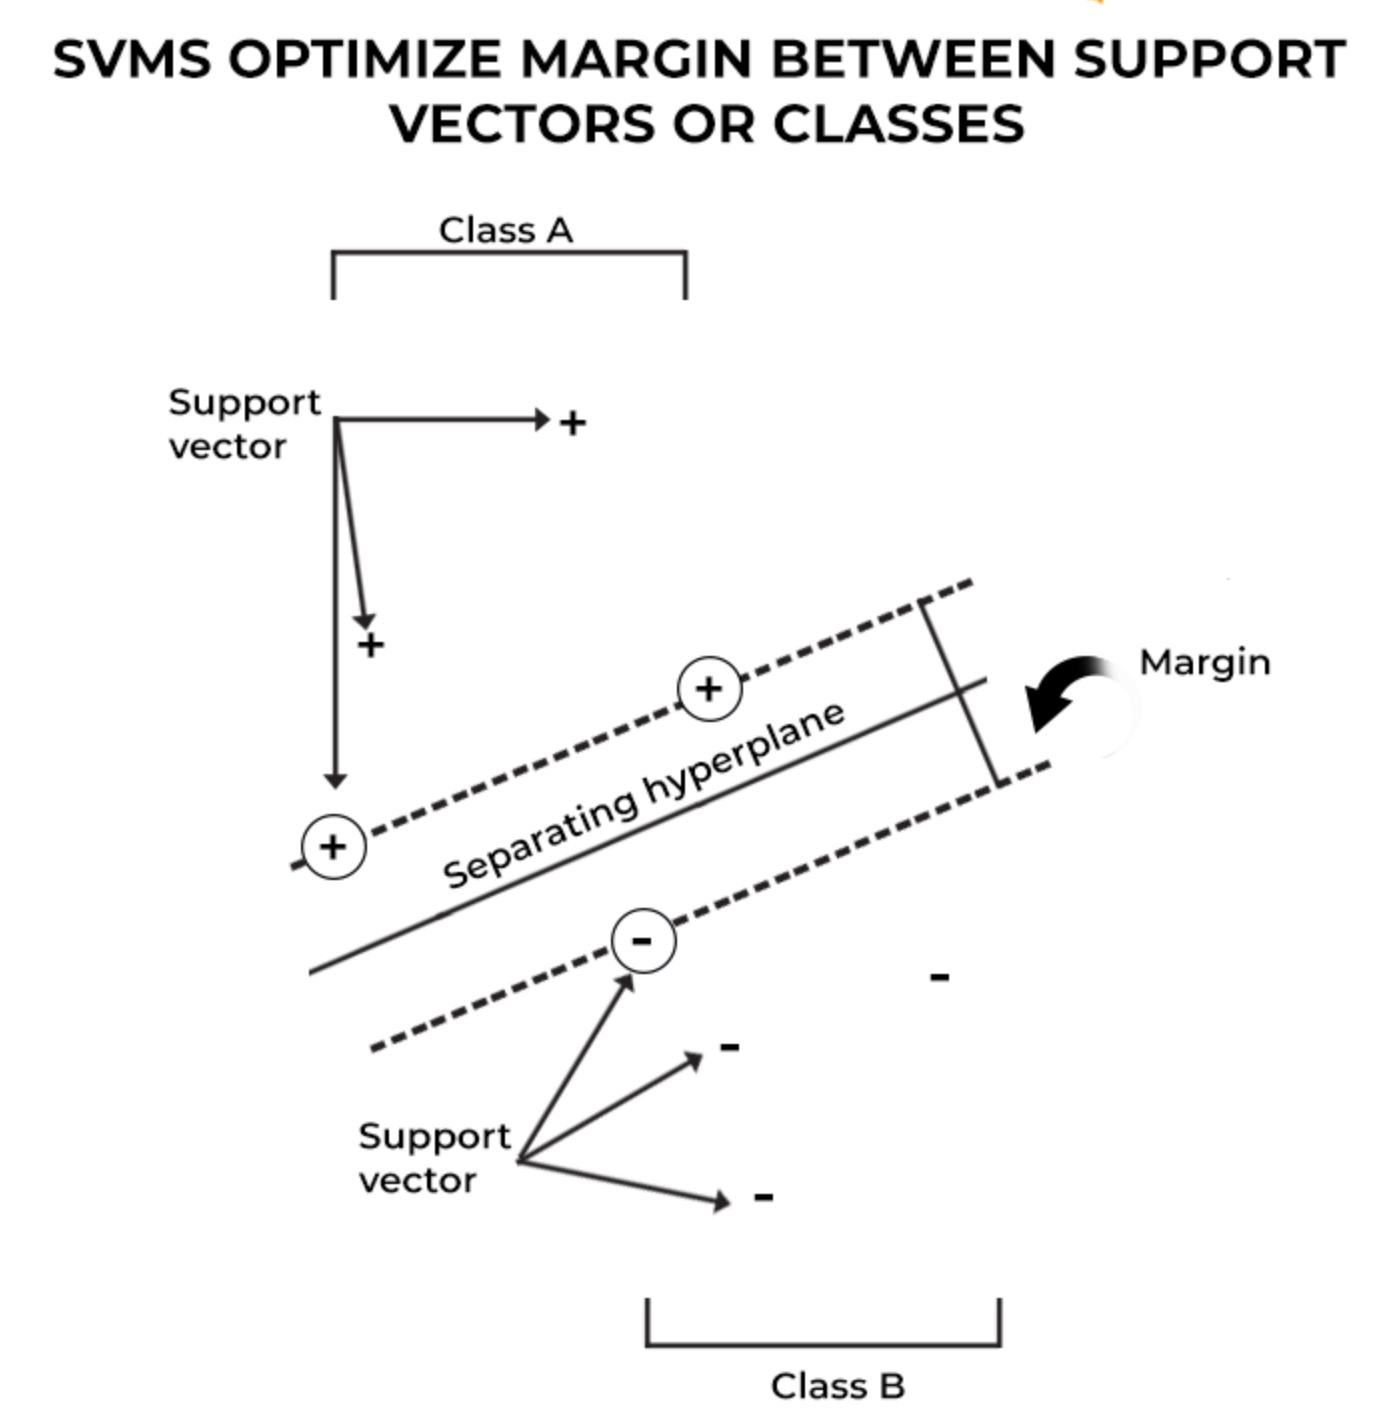
\includegraphics[width=0.5\textwidth]{SVMVisualization.png}}
    \caption{Visualization of hyperplane from SVM \cite{b6}.}
\end{figure}
As well, with modfications this strategy has been used to not only cover binary data but through using a method called a "kernel trick\cite{b6}" it is used on multidimensional data as well. 
Using this technique achieved very impressive accuracy levels on sentiment analysis of tweets according to other studies.
For example, in the study by Kavitha, Prasad Reddy, and Venkata Rao, it was observed that "SA [Sentiment Analysis] using SVM classifiers is varying between 90.1 and 94.8\%\cite{11}."
As well, in the study by Susmitha, Nikhul, Akhil, Kavitha, Reddy, and Shailaja, SVM had an accuracy percentage of 82\%\cite{b5}. 
Despite the success of this algorithm with studies seeing accuracy levels in the 90th percentile there is still a much smaller amount of knowledge on how a new style of algorithm would keep up.
A newer "self-supervised\cite{b7}" algorithm that has burst onto the scene is BERT.\newline 

BERT is an example of a self-supervised model. 
What this means is that it uses the data input to train on like a supervised algorithm however the training of the algorithm is done in an unsupervised fashion.
"The unsupervised problem is transformed into a supervised problem by auto-generating the labels\cite{b9}" for the supervised algorithm.
Analysis of study performed by Ionut-Alexandru and Stelian a hybrid of a "BERT and SVM Ensemble Model\cite{b8}" was used to detect emotions.
From this study they found very accurate results from combining the power of BERT and SVM with accuiracies in the 90th percentile.
From their results, the overall accuracy for their ensemble was 91\% \cite{b8}.
However their resulsts for BERT were 89\% \cite{b8}, which is very comparible to that of their ensemble.
These results can be seen in Figure 2.
This leads to the possibility of with different training and potentially more specific topics on tweets better results for BERTweet.

\begin{figure}[b]
    \centerline{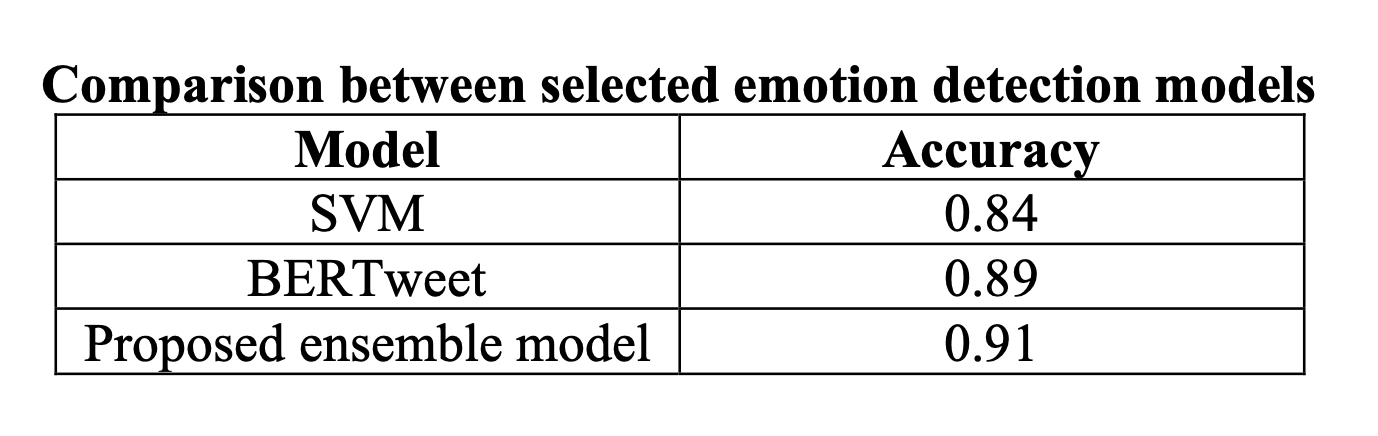
\includegraphics[width=0.5\textwidth]{BERTweetChartFromStudy.png}}
    \caption{Results from Study from Ionut-Alexandru and Stelian\cite{b8}}
\end{figure}

While these results are impressive the visualization of the results was not available other than through these tables.
In mentioned above by Samah, Jailani, Hamzah, Aminuddin, Abidin, and Ria, more time was spent on displaying the data to users nicely.
Several different types of charts including pie charts, bar graphs, and histograms were used to clearly visualize the data.
This makes understanding the algorithms decision on what the public feels on a certain topic much easier to understand compare to numbers in a chart.
An example of these charts can be seen in Figure 3. 
As well, in a study by Harshit D. Bhavani, they also created a web application to visualize the data\cite{b3}. 
However, both of these models have never used BERT or any other self-supervised algorithms with these visualizations.

\begin{figure*}[t]
    \centering
    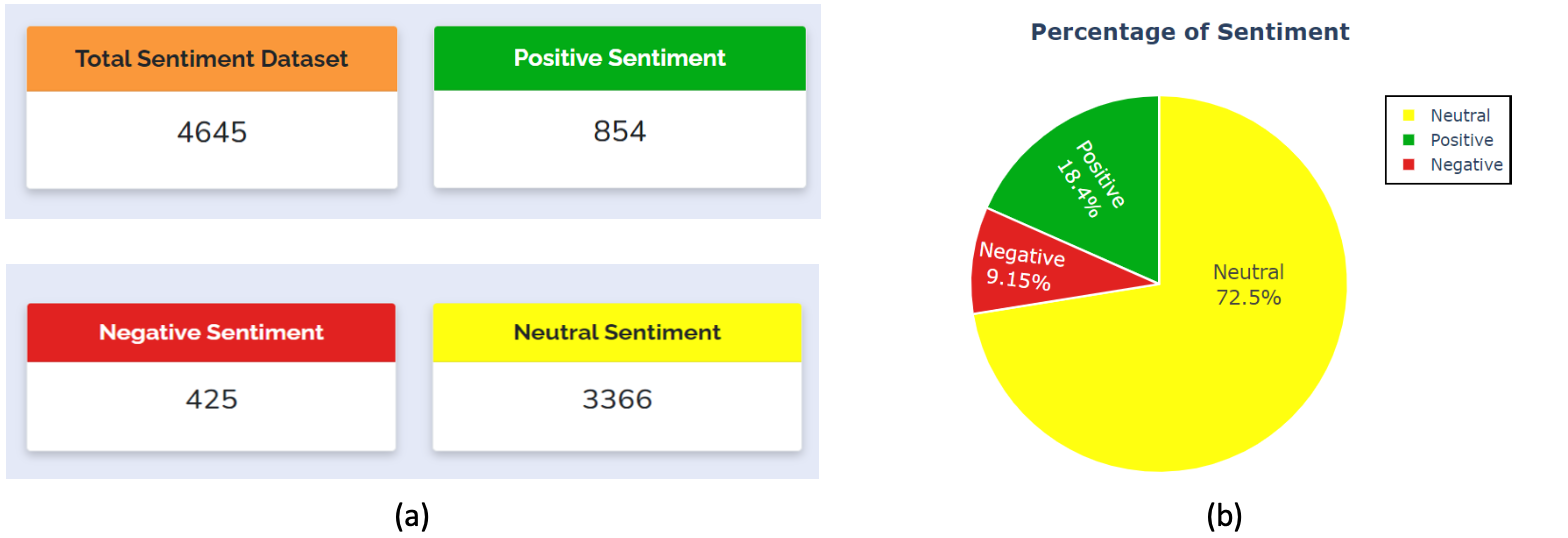
\includegraphics[width=0.8\textwidth]{BetterVisualizationsOfData.png}
    \caption{Example of visualization of data from study\cite{b2}}
\end{figure*}





\section{Proposed Methodology}
We will describe in detail what we plan to do for our implementation. 

\section{Dataset}
We will be giving an detailed desciption of our dataset
\begin{itemize}
    \item Description
    \item Weblinks
    \item Type of Data
    \item Statistics
\end{itemize}

\section{Implementaion Requirements}
Here we will be describing what tools we will need to implement the full stack experience

\section{Ease of Use}

\subsection{Maintaining the Integrity of the Specifications}

The IEEEtran class file is used to format your paper and style the text. All margins, 
column widths, line spaces, and text fonts are prescribed; please do not 
alter them. You may note peculiarities. For example, the head margin
measures proportionately more than is customary. This measurement 
and others are deliberate, using specifications that anticipate your paper 
as one part of the entire proceedings, and not as an independent document. 
Please do not revise any of the current designations.

\section{Prepare Your Paper Before Styling}
Before you begin to format your paper, first write and save the content as a 
separate text file. Complete all content and organizational editing before 
formatting. Please note sections \ref{AA}--\ref{SCM} below for more information on 
proofreading, spelling and grammar.

Keep your text and graphic files separate until after the text has been 
formatted and styled. Do not number text heads---{\LaTeX} will do that 
for you.

\subsection{Abbreviations and Acronyms}\label{AA}
Define abbreviations and acronyms the first time they are used in the text, 
even after they have been defined in the abstract. Abbreviations such as 
IEEE, SI, MKS, CGS, ac, dc, and rms do not have to be defined. Do not use 
abbreviations in the title or heads unless they are unavoidable.

\subsection{Units}
\begin{itemize}
\item Use either SI (MKS) or CGS as primary units. (SI units are encouraged.) English units may be used as secondary units (in parentheses). An exception would be the use of English units as identifiers in trade, such as ``3.5-inch disk drive''.
\item Avoid combining SI and CGS units, such as current in amperes and magnetic field in oersteds. This often leads to confusion because equations do not balance dimensionally. If you must use mixed units, clearly state the units for each quantity that you use in an equation.
\item Do not mix complete spellings and abbreviations of units: ``Wb/m\textsuperscript{2}'' or ``webers per square meter'', not ``webers/m\textsuperscript{2}''. Spell out units when they appear in text: ``. . . a few henries'', not ``. . . a few H''.
\item Use a zero before decimal points: ``0.25'', not ``.25''. Use ``cm\textsuperscript{3}'', not ``cc''.)
\end{itemize}

\subsection{Equations}
Number equations consecutively. To make your 
equations more compact, you may use the solidus (~/~), the exp function, or 
appropriate exponents. Italicize Roman symbols for quantities and variables, 
but not Greek symbols. Use a long dash rather than a hyphen for a minus 
sign. Punctuate equations with commas or periods when they are part of a 
sentence, as in:
\begin{equation}
a+b=\gamma\label{eq}
\end{equation}

Be sure that the 
symbols in your equation have been defined before or immediately following 
the equation. Use ``\eqref{eq}'', not ``Eq.~\eqref{eq}'' or ``equation \eqref{eq}'', except at 
the beginning of a sentence: ``Equation \eqref{eq} is . . .''

\subsection{\LaTeX-Specific Advice}

Please use ``soft'' (e.g., \verb|\eqref{Eq}|) cross references instead
of ``hard'' references (e.g., \verb|(1)|). That will make it possible
to combine sections, add equations, or change the order of figures or
citations without having to go through the file line by line.

Please don't use the \verb|{eqnarray}| equation environment. Use
\verb|{align}| or \verb|{IEEEeqnarray}| instead. The \verb|{eqnarray}|
environment leaves unsightly spaces around relation symbols.

Please note that the \verb|{subequations}| environment in {\LaTeX}
will increment the main equation counter even when there are no
equation numbers displayed. If you forget that, you might write an
article in which the equation numbers skip from (17) to (20), causing
the copy editors to wonder if you've discovered a new method of
counting.

{\BibTeX} does not work by magic. It doesn't get the bibliographic
data from thin air but from .bib files. If you use {\BibTeX} to produce a
bibliography you must send the .bib files. 

{\LaTeX} can't read your mind. If you assign the same label to a
subsubsection and a table, you might find that Table I has been cross
referenced as Table IV-B3. 

{\LaTeX} does not have precognitive abilities. If you put a
\verb|\label| command before the command that updates the counter it's
supposed to be using, the label will pick up the last counter to be
cross referenced instead. In particular, a \verb|\label| command
should not go before the caption of a figure or a table.

Do not use \verb|\nonumber| inside the \verb|{array}| environment. It
will not stop equation numbers inside \verb|{array}| (there won't be
any anyway) and it might stop a wanted equation number in the
surrounding equation.

\subsection{Some Common Mistakes}\label{SCM}
\begin{itemize}
\item The word ``data'' is plural, not singular.
\item The subscript for the permeability of vacuum $\mu_{0}$, and other common scientific constants, is zero with subscript formatting, not a lowercase letter ``o''.
\item In American English, commas, semicolons, periods, question and exclamation marks are located within quotation marks only when a complete thought or name is cited, such as a title or full quotation. When quotation marks are used, instead of a bold or italic typeface, to highlight a word or phrase, punctuation should appear outside of the quotation marks. A parenthetical phrase or statement at the end of a sentence is punctuated outside of the closing parenthesis (like this). (A parenthetical sentence is punctuated within the parentheses.)
\item A graph within a graph is an ``inset'', not an ``insert''. The word alternatively is preferred to the word ``alternately'' (unless you really mean something that alternates).
\item Do not use the word ``essentially'' to mean ``approximately'' or ``effectively''.
\item In your paper title, if the words ``that uses'' can accurately replace the word ``using'', capitalize the ``u''; if not, keep using lower-cased.
\item Be aware of the different meanings of the homophones ``affect'' and ``effect'', ``complement'' and ``compliment'', ``discreet'' and ``discrete'', ``principal'' and ``principle''.
\item Do not confuse ``imply'' and ``infer''.
\item The prefix ``non'' is not a word; it should be joined to the word it modifies, usually without a hyphen.
\item There is no period after the ``et'' in the Latin abbreviation ``et al.''.
\item The abbreviation ``i.e.'' means ``that is'', and the abbreviation ``e.g.'' means ``for example''.
\end{itemize}
An excellent style manual for science writers is \cite{b7}.

\subsection{Authors and Affiliations}
\textbf{The class file is designed for, but not limited to, six authors.} A 
minimum of one author is required for all conference articles. Author names 
should be listed starting from left to right and then moving down to the 
next line. This is the author sequence that will be used in future citations 
and by indexing services. Names should not be listed in columns nor group by 
affiliation. Please keep your affiliations as succinct as possible (for 
example, do not differentiate among departments of the same organization).

\subsection{Identify the Headings}
Headings, or heads, are organizational devices that guide the reader through 
your paper. There are two types: component heads and text heads.

Component heads identify the different components of your paper and are not 
topically subordinate to each other. Examples include Acknowledgments and 
References and, for these, the correct style to use is ``Heading 5''. Use 
``figure caption'' for your Figure captions, and ``table head'' for your 
table title. Run-in heads, such as ``Abstract'', will require you to apply a 
style (in this case, italic) in addition to the style provided by the drop 
down menu to differentiate the head from the text.

Text heads organize the topics on a relational, hierarchical basis. For 
example, the paper title is the primary text head because all subsequent 
material relates and elaborates on this one topic. If there are two or more 
sub-topics, the next level head (uppercase Roman numerals) should be used 
and, conversely, if there are not at least two sub-topics, then no subheads 
should be introduced.

\subsection{Figures and Tables}
\paragraph{Positioning Figures and Tables} Place figures and tables at the top and 
bottom of columns. Avoid placing them in the middle of columns. Large 
figures and tables may span across both columns. Figure captions should be 
below the figures; table heads should appear above the tables. Insert 
figures and tables after they are cited in the text. Use the abbreviation 
``Fig.~\ref{fig}'', even at the beginning of a sentence.

\begin{table}[htbp]
\caption{Table Type Styles}
\begin{center}
\begin{tabular}{|c|c|c|c|}
\hline
\textbf{Table}&\multicolumn{3}{|c|}{\textbf{Table Column Head}} \\
\cline{2-4} 
\textbf{Head} & \textbf{\textit{Table column subhead}}& \textbf{\textit{Subhead}}& \textbf{\textit{Subhead}} \\
\hline
copy& More table copy$^{\mathrm{a}}$& &  \\
\hline
\multicolumn{4}{l}{$^{\mathrm{a}}$Sample of a Table footnote.}
\end{tabular}
\label{tab1}
\end{center}
\end{table}

Figure Labels: Use 8 point Times New Roman for Figure labels. Use words 
rather than symbols or abbreviations when writing Figure axis labels to 
avoid confusing the reader. As an example, write the quantity 
``Magnetization'', or ``Magnetization, M'', not just ``M''. If including 
units in the label, present them within parentheses. Do not label axes only 
with units. In the example, write ``Magnetization (A/m)'' or ``Magnetization 
\{A[m(1)]\}'', not just ``A/m''. Do not label axes with a ratio of 
quantities and units. For example, write ``Temperature (K)'', not 
``Temperature/K''.

\section*{Acknowledgment}

The preferred spelling of the word ``acknowledgment'' in America is without 
an ``e'' after the ``g''. Avoid the stilted expression ``one of us (R. B. 
G.) thanks $\ldots$''. Instead, try ``R. B. G. thanks$\ldots$''. Put sponsor 
acknowledgments in the unnumbered footnote on the first page.

\section*{References}

Please number citations consecutively within brackets \cite{b1}. The 
sentence punctuation follows the bracket \cite{b2}. Refer simply to the reference 
number, as in \cite{b3}---do not use ``Ref. \cite{b3}'' or ``reference \cite{b3}'' except at 
the beginning of a sentence: ``Reference \cite{b3} was the first $\ldots$''

Number footnotes separately in superscripts. Place the actual footnote at 
the bottom of the column in which it was cited. Do not put footnotes in the 
abstract or reference list. Use letters for table footnotes.

Unless there are six authors or more give all authors' names; do not use 
``et al.''. Papers that have not been published, even if they have been 
submitted for publication, should be cited as ``unpublished'' \cite{b4}. Papers 
that have been accepted for publication should be cited as ``in press'' \cite{b5}. 
Capitalize only the first word in a paper title, except for proper nouns and 
element symbols.

For papers published in translation journals, please give the English 
citation first, followed by the original foreign-language citation \cite{b6}.

\begin{thebibliography}{00}
\bibitem{b1} \url{https://link.springer.com/article/10.1007/s13278-022-01000-9}
\bibitem{b2} \url{https://semarakilmu.com.my/journals/index.php/applied_sciences_eng_tech/article/view/3281/3455}
\bibitem{b3} \url{https://ojs.wiserpub.com/index.php/CCDS/article/view/1827}
\bibitem{b4} \url{https://link.springer.com/chapter/10.1007/978-981-19-8865-3_12}
\bibitem{b5} \url{https://ieeexplore.ieee.org/abstract/document/10084278?casa_token=GlPE_azfZjoAAAAA:Uk5ZcMsTMxXDFkBargYNGNlRHcoa9OyNy9uMpXBAo3gc70oD59nl6fnJw4J_Bts1-pUa8mO_}
\bibitem{b6} \url{https://www.spiceworks.com/tech/big-data/articles/what-is-support-vector-machine/#:~:text=A%20support%20vector%20machine%20(SVM)%20is%20a%20machine%20learning%20algorithm,classes%2C%20labels%2C%20or%20outputs.}
\bibitem{b7} \url{https://www.projectpro.io/article/bert-nlp-model-explained/558}
\bibitem{b8} \url{https://arxiv.org/pdf/2208.04547.pdf}
\bibitem{b9} \url{https://neptune.ai/blog/self-supervised-learning#:~:text=Self%2Dsupervised%20learning%20is%20a,as%20predictive%20or%20pretext%20learning.}
\end{thebibliography}
\vspace{12pt}
\color{red}
IEEE conference templtes contain guidance text for composing and formatting conference papers. Please ensure that all template text is removed from your conference paper prior to submission to the conference. Failure to remove the template text from your paper may result in your paper not being published.

\end{document}